\section{Model}
\label{sec:model}
\begin{quotation}
	"All models are wrong; some models are useful" - George Box
\end{quotation}

% Sanders~\cite{sanders2009security} argues that existing security metrics should be integrated to provide a comprehensive, quantified view of systems through their lifecycle.  

 If we are to measure and understand how security practice use influences security outcomes, we need to account for the other influences on security outcomes. We recognize that both software quality factors, such as code size, and factors external to software development, such as the amount of money managed by the software, influence security outcomes. Software quality and software usage context factors are multi-faceted, with multiple contributing causes. For example, software quality attributes with effects on security outcomes include code size ~\cite{alhazmi2007measuring}, code churn ~\cite{shin2011evaluating}, and language ~\cite{ray2014a}. Software usage context factors are not limited to the amount of money managed directly by software; attackers also focus on users and on machines. 
 
 We seek a model of the factors influencing security outcomes in software development to enable assessment of how varying security practice use affects those outcomes. 
 
 The Common Criteria (CC) introduction~\cite{common2012common} lists a set of \textbf{security concepts} (concepts bolded) and relationships, summarized as follows:
 \begin{itemize}
 	\item  Owners value \textbf{Assets}, and seeking to minimize \textbf{Risk}, impose \textbf{Countermeasures} to reduce \textbf{Risk}.
 	\item Threat Agents give rise to \textbf{Threats} that affect \textbf{Assets} and increase \textbf{Risk}.
 \end{itemize}
 
 Considering the CC concepts, we propose a four construct structural model, described below, to capture the distinction between software quality factors and software usage factors when measuring practice usage's effect on security outcomes. We expect our model to be useful in assessing the relative impact of software quality factors and software usage factors on security outcomes, and in assessing the effect of security practice adherence on software quality. Given the complexity of software security, we expect that this initial model will be wrong to some degree, and we will use our data collection to evaluate the model and to evaluate possible refinements.

We have theorized relationships between measurement variables and each construct in our model, for example we theorize that the already mentioned code size and code churn metrics influence Software Risk. We present our list of measurements in Section \ref{sec:model_measurement}.

\subsection{Structural Model Constructs}
 \label{sec:model_structual}
In this section, we define the Software Risk, Asset Impact, Adherence, and Outcomes constructs, and the relationships we expect between each construct. 

To make claims about how security practices affect security outcomes, we need to account for other influences on security outcomes.

\subsubsection{Software Risk}
Software Risk (measurement of CC \textbf{Risk} potential) represents the characteristics of the software under the control of the development team that are associated with Outcomes. In the case of software vulnerabilities, for example, high code churn and defect-prone languages have been correlated with vulnerabilities.

\subsubsection{Asset Impact}
Asset Impact (CC \textbf{Assets}) represents the characteristics of the software's purpose and usage context that are associated with attacker interest. One component of attacker interest is the value of the objects managed by the software. For example, we hypothesize that software tracking valuable or sensitive data, such as PII or credit card data is more likely to be attacked than software tracking, say, baseball scores. As another example, attacker control over a machine enables the machine's participation in a botnet, making the number of machines on which a piece of software runs a consideration in evaluating the software's Asset Impact.

\subsubsection{Adherence}
\label{sec:model_contruct_adherence}
Adherence (CC \textbf{Countermeasures}) represents the efforts the team takes to prevent and discover vulnerabilities. We adapt an IEEE definition of practice~\cite{ieee1990glossary} `3. a specific type of professional or management activity that contributes to 
the execution of a process and that may employ one or more techniques and tools' to define a software development security practice to be an action a software development team member takes to prevent, identify, or resolve a vulnerability, possibly guided by a tool or reference. We measure the Adherence construct in terms of the frequency  of security practice use by the team.  
% emails - spec
% commit messages - code
% tests - test
% issues - ops
% documentation - spec

\subsubsection{Outcomes}
\label{sec:model_contruct_outcome}
The Outcomes  ((measurement of CC \textbf{Risk} realized)) construct represents security-related events associated with a piece of software over the course of the software's life cycle. Security-related events may be positive or negative. 
\begin{itemize}
	\item Positive outcomes: Meneely~\cite{meneely2016security} observes that security is negatively defined, the absence of issues in a system's confidentiality, integrity, and availability. We posit that measures of the absence of security issues over time would prove valuable in management, development team, and user assessment of software. However, we are aware of no such measures.
	\item Negative outcomes: At present, the presence of security issues, termed vulnerabilities, is the most common means of measuring security in software~\cite{morrison2014mapping}. Following Krsul~\cite{krsul1998software} and Ozment~\cite{ozment2007vulnerability}, we define a software vulnerability as “an instance of a mistake in the specification, development, or configuration of software such that its execution can violate the explicit or implicit security policy." We distinguish between undiscovered (`latent') and discovered (`manifest') security issues. We, further, distinguish between vulnerabilities identified after the software is released (`Post-release'), and vulnerabilities identified before the software is released (`Pre-release'). 
\end{itemize} 

We measure the Outcomes construct in terms of manifest vulnerabilities and the timing of their discovery and resolution. Low total values for manifest vulnerabilities are preferable, and a high proportion of vulnerabilities discovered pre-release rather than post-release is also preferable. 

\subsection{Structural Model Relationships}
We hypothesize that the four constructs are related as follows:
\begin{itemize}
	\item \textbf{H1} Asset Impact is positively associated with negative Security Outcomes
	\item \textbf{H2} Software Risk is positively associated with negative Security Outcomes
	\item \textbf{H3} Practice Adherence is negatively associated with Software Risk 	
\end{itemize}

For example, a carefully-written piece of widely-used software that manages financial data (high Asset Impact, low Software Risk) may have poorer Outcomes than a less well written baseball scores program used by a few hundred users (low Asset Impact, high Software Risk). In an ideal world, we would expect Adherence to be correlated with Asset Impact, as teams adopted security practices in proportion to the security needs of their software, its usage context, and their users. In practice, for example in the case of the CloudBleed example from the introduction of the paper, users (especially attackers) sometimes surprise development teams in the uses of their software, unexpectedly increasing the software's Asset Impact out of proportion to the team's Adherence. 

In this work, we use the lavaan~\cite{roseel2012lavaan} model syntax to express the modeled constructs and relationships.  We now introduce the syntax in both its textual and graphical representations, and explain the semantics of each syntax element.

Figure~\ref{fig:model_constructs} depicts the constructs and their relationships.  Each circle in the figure represents a construct, modeled as a `latent variable'. We model the constructs using latent variables to indicate that our measures for each construct are aggregates of observed variables containing some level of measurement error with respect to the construct~\cite{kline2015principles,borsboom2008latent}. 

Directed edges from circles to other circles, for example the arrow from AssetImpact to Outcomes in Figure \ref{fig:model_constructs}, represent a source latent variable's effect on the target latent variable. The size of the effect is established by determining a parameter estimate for the edge. A one unit change on the source side of the relationship is associated with a parameter-estimate-sized-change on the target side of the relationship, in the direction of the sign of the parameter estimate. In the lavaan software we use in this paper, these regression relationships between latent variables are specified using the $\sim$  operator (see Table \ref{tab:model_lavaan_syntax}), for example $Outcomes ~ SoftwareRisk + AssetImpact$ (SoftwareRisk is also modeled as affecting Outcomes).   Establishing a parameter estimate for this relationship allows us to test hypothesis \textbf{H1} Asset Impact is positively associated with negative Security Outcomes.

Dual arrows between circles/constructs, for example between Adherence and AssetImpact in Figure \ref{fig:model_constructs}, represent covariances between the constructs, implying that a relationship exists, but that the direction of influence is not specified. Dual arrows starting and ending at the same variable indicate residual variance, the amount of variation in the observed variable not explained by the model. In the lavaan software we use in this paper, these covariance relationships are specified using the $\sim\sim$ operator.

Each square in Figure \ref{fig:model_example_syntax_asmeasuredby} represents a measurement variable associated with each construct. Directed edges (single arrows) from circles to squares, for example from SoftwareRisk to SLOC as shown in Figure \ref{fig:model_example_syntax_asmeasuredby}, represent that a construct `is measured by' a measurement variable relationship. The parameter estimate on these relationships represents the sign and magnitude of the relative contribution of the measurement variable to the construct value.The `is measured by' relationships are specified as follows: $LatentVariable =\sim MeasuredVariable1 [+ MeasuredVariable2]$. We present the list of measurements for each construct in the measurement guidebook~\footnote{http://pjmorris.github.io/Security-Practices-Evaluation-Framework/guidebook.html}, and we present the measurement variables that we select from each dataset in the case studies.  

Dashed lines indicate fixed estimates, set either by the modeler, or by the software. We have two examples of modeled fixed parameters in our structural model: We specify the absence of a direct relationship between Asset Impact and Software Risk (syntax: $SoftwareRisk \sim\sim 0*AssetImpact$), as we expect the constructs to be independent of each other. We specify the absence of a direct relationship between Adherence and Outcomes, as we expect Adherence to affect Outcomes through being moderated by overall Software Risk. The remaining dashed lines are estimates fixed by the software, where it has estimated starting values in the course of solving the system of equations expressed by the model. 

The lavaan model syntax for the complete set of structural model constructs and relationships (but not the measurement model) is as follows:
 
 \begin{align*}
 SoftwareRisk =\sim SoftwareContextFactors\\
 AssetImpact =\sim AssetContextFactors\\
 Outcomes =\sim OutcomesContextFactors\\ 
 Adherence =\sim AdherenceContextFactors\\
 Outcomes \sim SoftwareRisk + AssetImpact\\
 SoftwareRisk \sim Adherence\\
 \\
 AssetImpact \sim\sim  Adherence\\
 SoftwareRisk \sim\sim 0*AssetImpact\\
 Adherence \sim\sim 0*Outcomes\\
 \end{align*}
 
 \begin{figure}
 	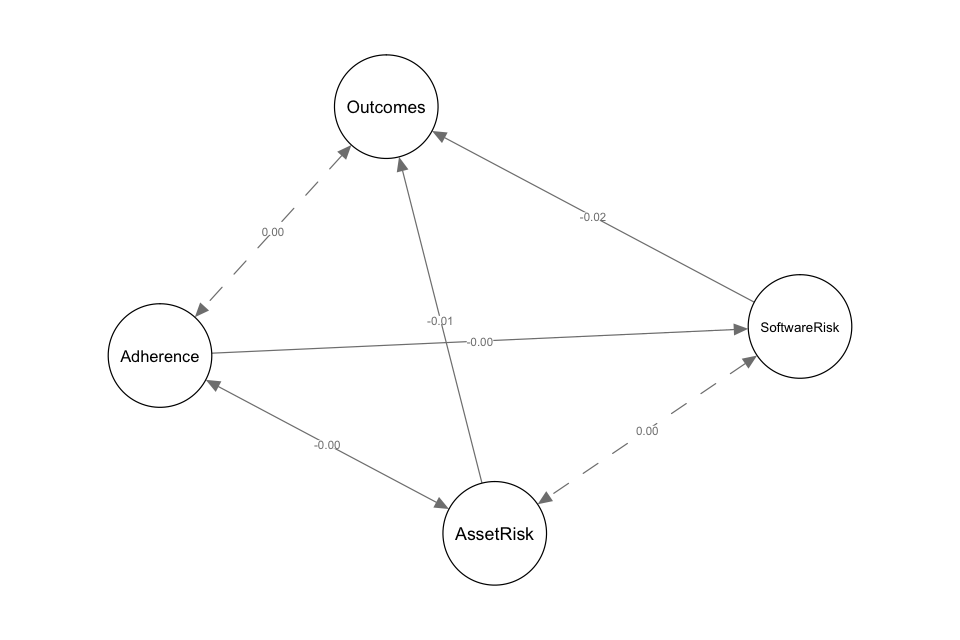
\includegraphics[width=\columnwidth]{modelzeroB.png}
 	\caption{Structural and Measurement Model Overview}
 	\label{fig:model_constructs}
 \end{figure}
  
\begin{table*}[!htbp] \centering 
	\caption{Lavaan Syntax} 
	\label{tab:model_lavaan_syntax} 
	\begin{small}
		\begin{tabular}{p{.75cm}p{1.25cm}p{1cm}p{5cm}p{4cm}} 
			&&&&\\[-1.8ex]\hline 
			\hline&&&& \\[-1.8ex] 
			Syntax & Symbol & Name & Description & Example \\ 
			\hline &&&&\\[-1.8ex]  
			$=\sim$	& $\bigcirc \rightarrow \Box$ & is measured by & $=\sim$ specifies how a latent variable (left side) is measured by the constituent variables listed on the right side & $SoftwareRisk =\sim SLOC + Churn$\\	
			 $\sim$ & $\bigcirc \leftarrow \bigcirc$ & regression & $\sim$ specifies a regression of the dependent variable on the left-hand side to the independent variables on the right hand side of the expression. & Outcomes $\sim$ SoftwareRisk $+$ AssetImpact  \\	
			 $\sim\sim$ & $\bigcirc \leftrightarrow \bigcirc$ $\Box \leftrightarrow \Box$ & undirected covariance & model a covariance relationship, but leave the direction of influence unspecified & $Adherence \sim\sim Adherence$\\
			\hline &&&&\\[-1.8ex] 
			\hline &&&&\\[-1.8ex] 
		\end{tabular} 
	\end{small}
\end{table*} 


\begin{figure*}
	\centering
%	\begin{subfigure}{.5\textwidth}
		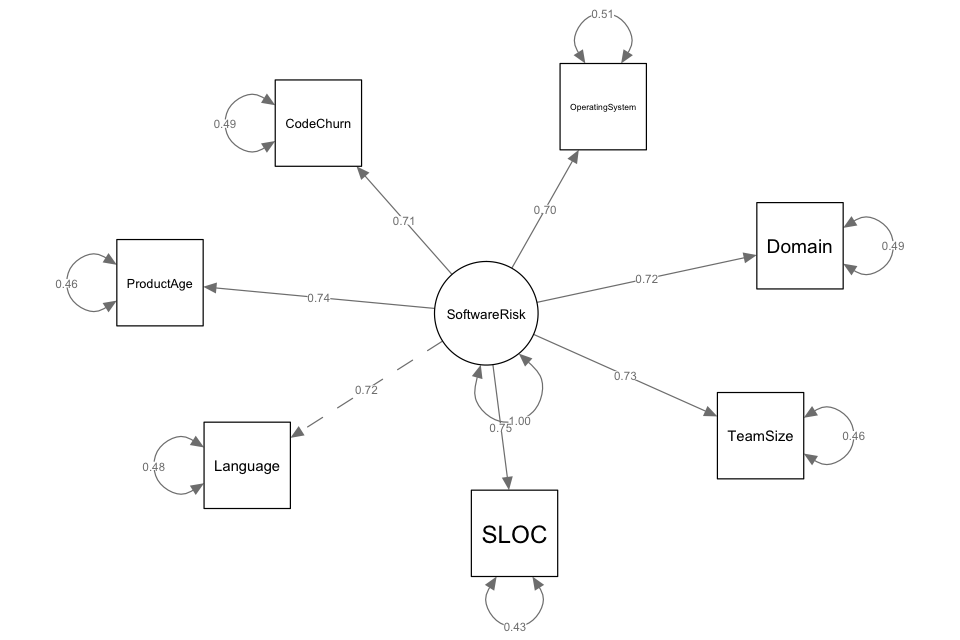
\includegraphics[width=1\textwidth]{syntax_swrisk_asmeasuredby.png}
		\caption{Graphical display of lavaan syntax for SoftwareRisk $=\sim$ Theorized measurement variables from Table  \ref{tab:model_spef_metrics}}
		\label{fig:model_example_syntax_asmeasuredby}	
%	\end{subfigure}%
%	\begin{subfigure}{.5\textwidth}		
%		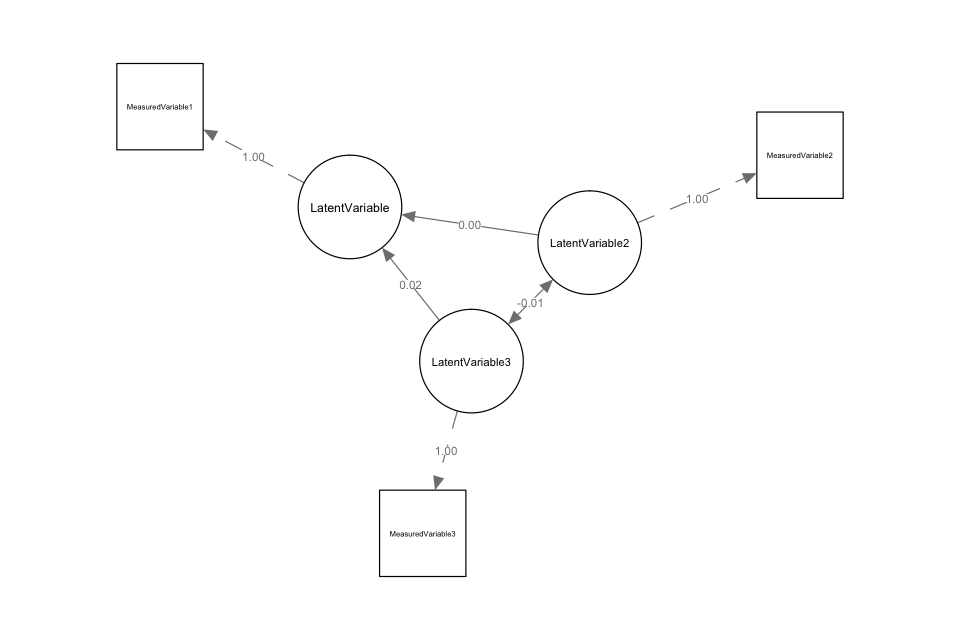
\includegraphics[width=.5\columnwidth]{syntax_latentregress.png}
%		\caption{Graphical display of lavaan syntax for $LatentVariable \sim LatentVariable2 + LatentVariable3$ (with measured variables)}
%		\label{fig:model_example_syntax_latentregress}	
%	\end{subfigure}		
\end{figure*}

%\begin{figure}
% \includegraphics[width=\columnwidth]{modelcaoscto}
%	\caption{Model Constructs and Sub-Constructs}
%	\label{fig:model_constructs_phases}
%\end{figure}

\subsection{Measurement Model: Metrics, Variables, and Relationships}
\label{sec:model_measurement}
%~\cite{morrison2014mapping}
%~\cite{morrison2016spefsite}
Through literature review~\cite{morrison2014mapping} and analysis~\cite{morrison2017surveying,morrison2017measuring}, we have developed a set of measurements that we expect to capture security-related constructs for software development. To collect empirical data, we have developed a data collection framework for the measurement model, available online (URL on request). In Table \ref{tab:model_spef_metrics}, we name each data element, give our hypothesis about its relationship to the structural model construct, and cite a rationale for the data element's presence. 
		
\begin{table*}[!htbp] \centering 
	\caption{Model Metrics and Hypotheses} 
	\label{tab:model_spef_metrics} 
	\begin{small}
		\begin{tabular}{@{\extracolsep{5pt}}p{3cm}p{1cm}p{2cm}p{10cm}} 
			\\[-1.8ex]\hline 
		\hline \\[-1.8ex] 
		Metric & \multicolumn{1}{c}{Effect} & \multicolumn{1}{c}{Construct} & \multicolumn{1}{c}{Rationale} \\ 
		\hline \\[-1.8ex]  
			Language	& influences &	Software Risk &   Ray et al. ~\cite{ray2014a} and Walden et al. ~\cite{walden2010idea} found small but significant effects of programming language on software quality. \\
			Operating System	& influences &	Software Risk & \\	
			Domain &	influences &	Software Risk	 & Different risks are associated with different software domains~\cite{williams2004xpef,jones2000software} \\
			Product Age	& increases &	Software Risk & Kaminsky et al.~\cite{kaminsky2011showing} and Morrison et al.~\cite{morrison2015challenges} have found evidence of code age effects on the presence of vulnerabilities. \\
			
			Source Lines of Code (SLOC)	& influences	& Software Risk & Source code size is correlated with vulnerabilities ~\cite{shin2011evaluating}, ~\cite{alhazmi2007measuring}. \\
			Churn &	increases &	Software Risk  &  Code churn is correlated with vulnerabilities ~\cite{shin2011evaluating}.\\
			Team Size	& influences	& Software Risk & Shin et al. ~\cite{shin2011evaluating} and Zimmermann et al. ~\cite{zimmerman2010searching} found correlations between team size and vulnerabilities. \\			
			\hline \\[-1.8ex] 
			Number of Machines &	increases &	Asset Impact & (Proposed) The market for machine time on botnets suggests that the number of machines a piece of software runs on increases the software's desirability to attackers. \\
			Number of Identities &	increases &	Asset Impact	 &  (Proposed) The market for personal identities and credit card information suggests that the number of identities a piece of software manages increases the software's desirability to attackers.\\
			Number of Dollars &	increases &	Asset Impact	 & (Proposed) The amount of financial resources a piece of software manages increases the software's desirability to attackers\\
			Source Code Availability	& influences &	Asset Impact & While Anderson ~\cite{anderson2002security} argues that attack and defense
			are helped equally by the open vs. closed source decision, we collect this data to enable further analysis.  \\
			Confidentiality, Integrity, Availability Requirements &	increases &	Asset Impact	& Explicit security requirements for a piece of software imply a higher level of Asset Impact for the software ~\cite{mell2007complete}. \\
			\hline \\[-1.8ex]
			Team Location &	influences &	Adherence	& (Proposed)  Kocaguneli ~\cite{kocaguneli2013distributed} reports on the debate over the effect of team location on software quality, collecting data on team location supports study of its effect. \\
			Methodology	& influences &	Adherence	& Different risks are associated with different software methodologies~\cite{williams2004xpef,jones2000software} \\
			Apply Data Classification Scheme & increases & 	Adherence & (Proposed) Identifying data in need of protection supports reducing Software Risk~\cite{morrison2017surveying}.\\	
			Apply Security Requirements	&	increases	&	Adherence & (Proposed)  supports reducing Software Risk[ref Riaz, etc] ~\cite{morrison2017surveying}.\\
			Perform Threat Modeling &	increases &	Adherence &(Proposed) Identification and analysis of threats supports reducing Software Risk~\cite{morrison2017surveying}. \\	
			Document Technical Stack &	increases &	Adherence & (Proposed) Understanding and controlling platform and dependency characteristics supports reducing Software Risk~\cite{morrison2017surveying}.\\	
			Apply Secure Coding Standards &	increases	& Adherence & (Proposed)  Avoiding known implementation erros supports reducing Software Risk~\cite{morrison2017surveying}.\\
			Apply Security Tooling &	increases &	Adherence & (Proposed)  Automated static and dynamic security analysis supports reducing Software Risk~\cite{morrison2017surveying}.\\
			Perform Security Testing &	increases &	Adherence & (Proposed)  Explicit validation of security requirement fulfillment supports reducing Software Risk~\cite{morrison2017surveying}.\\	
			Perform Penetration Testing &	increases &	Adherence	& (Proposed)  Exploratory testing of security properties supports reducing Software Risk~\cite{morrison2017surveying}.\\
			Perform Security Review &	increases &	Adherence	&  McIntosh et al. ~\cite{mcintosh2014the} observed lower defects for highly reviewed components. Meneely et al. ~\cite{meneely2014empirical} observed lower vulnerabilities for components with experienced reviwers. \\
			Publish Operations Guide &	increases	& Adherence & (Proposed) Documenting software security characteristics and configuration requirements supports reducing Software Risk~\cite{morrison2017surveying}.\\
			Track Vulnerabilities &	increases &	Adherence & (Proposed) Incident recognition and response supports reducing Software Risk~\cite{morrison2017surveying}.\\	
			Improve Development Process &	increases &	Adherence & (Proposed)  Adoption and adaptation of security tools and techniques based on experience supports reducing Software Risk~\cite{morrison2017surveying}.\\	
			Perform Security Training &	increases &	Adherence	& (Proposed) Development team knowledge of security risks and mitigations supports reducing Software Risk~\cite{morrison2017surveying}.\\		
			\hline \\[-1.8ex] 
			Vulnerabilities	& represent & Outcomes &  Vulnerabilities are, by definition, a negative security outcome, e.g. ~\cite{alhazmi2007measuring}.\\
			Defects & represent & Outcomes	& \\		
			\hline \\[-1.8ex] 
			\hline \\[-1.8ex] 
		\end{tabular} 
	\end{small}
\end{table*} 
%\subsubsection{Software Risk}
%\subsubsection{Asset Impact}
%\subsubsection{Practice Adherence}
%\subsubsection{Security Outcomes}